
\documentclass[12pt]{article}
\setlength\parindent{0pt}
\usepackage{fullpage}
\usepackage{amsmath}
\usepackage[margin=0.5in, paperwidth=13.5in, paperheight=8.4in]{geometry}
\usepackage{graphicx}
\setlength{\parskip}{4mm}
\def\LL{\left\langle}   % left angle bracket
\def\RR{\right\rangle}  % right angle bracket
\def\LP{\left(}         % left parenthesis
\def\RP{\right)}        % right parenthesis
\def\LB{\left\{}        % left curly bracket
\def\RB{\right\}}       % right curly bracket
\def\PAR#1#2{ {{\partial #1}\over{\partial #2}} }
\def\PARTWO#1#2{ {{\partial^2 #1}\over{\partial #2}^2} }
\def\PARTWOMIX#1#2#3{ {{\partial^2 #1}\over{\partial #2 \partial #3}} }
\newcommand{\BE}{\begin{displaymath}}
\newcommand{\EE}{\end{displaymath}}
\newcommand{\BC}{\begin{center}}
\newcommand{\EC}{\end{center}}
\newcommand{\BNE}{\begin{equation}}
\newcommand{\ENE}{\end{equation}}
\newcommand{\BEA}{\begin{eqnarray}}
\newcommand{\EEA}{\nonumber\end{eqnarray}}
\newcommand{\EL}{\nonumber\\}
\newcommand{\la}[1]{\label{#1}}
\newcommand{\ie}{{\em i.e.\ }}
\newcommand{\eg}{{\em e.\,g.\ }}
\newcommand{\cf}{cf.\ }
\newcommand{\etc}{etc.\ }
\newcommand{\Tr}{{\rm tr}}
\newcommand{\etal}{{\it et al.}}
\newcommand{\OL}[1]{\overline{#1}\ } % overline
\newcommand{\OLL}[1]{\overline{\overline{#1}}\ } % double overline
\newcommand{\OON}{\frac{1}{N}} % "one over N"
\newcommand{\OOX}[1]{\frac{1}{#1}} % "one over X"

\pagenumbering{gobble}

\begin{document}
\Large
\centerline{\sc{Recitation Exercises}}
\normalsize
\centerline{\sc{Wednesday, 28 April}}

You should work on problems 2 and 4 from Homework 9 with your group. (Problem 2 is quite simple, but is nuanced -- you should talk to a coach about it if you are stuck.) 

The following two problems from previous exams (appearing on the next pages) will also be good practice for you.


\newpage


A meter stick is elevated at a $\theta=30^\circ$ angle. A spool consists of a cylinder of radius 2 cm with two disks affixed on either end; the disks have a
radius of 10 cm. The cylinder is very light; you may assume all of the mass of the spool is in the disks. The spool is placed at the top of the meter stick
so that the cylinder is touching the stick; when it is released, it rolls without slipping to the bottom. \it (The moment of inertia of a disk is $\frac{1}{2}mr^2)$. \rm

In this problem, you will calculate the speed of the spool at the bottom.

\small

You may solve this problem in either symbols or numbers.
If you use symbols, you must tell me the physical values of each symbol that you use (for instance: ``$r=2$ cm''). If you use numbers, you {\it must} retain the
units (i.e. write ``10 cm'', not ``10''.)

\normalsize\bigskip\bigskip

\begin{minipage}{0.2\textwidth}
	\BC
	\it (Side view)
	
	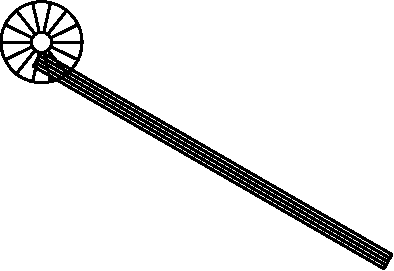
\includegraphics[width=\textwidth]{sideview-crop.pdf}
	\EC
\end{minipage}
\begin{minipage}{0.3\textwidth}
	\BC
	\it (Rear view)
	
	\vspace{1cm}
	
	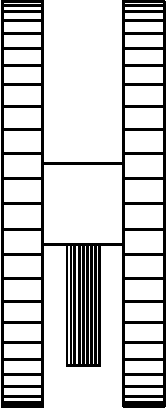
\includegraphics[width=0.15\textwidth]{rearview-crop.pdf}
	\EC
\end{minipage}
\begin{minipage}{0.5\textwidth}

a) What is the relation between the spool's translational velocity $v$ and its angular velocity $\omega$? Remember that if you use variables here, you must tell
me their physical values.
	\vspace{1in}
	
\end{minipage}	
\vspace{0.3in}


b) Recall that the total work  done by the force of static friction as the spool rolls downward is {\it zero}. Calculate the velocity of the spool at the bottom.

\newpage


A spring has spring constant $k$. One end is fixed, and the other end is attached to a mass $m$, which is free to move horizontally along a table. The mass slides over the table with a coefficient of friction $\mu_k$.

The spring is compressed a distance $d$ from its equilibrium point and released. When the spring is released, it will push the mass to the right, until it reaches some other distance $d_f$ past the equilibrium point.

\bigskip

%\centerline{\hspace{0.2\textwidth}Before\hspace{0.4\textwidth}After\hspace{0.2\textwidth}}

\centerline{
	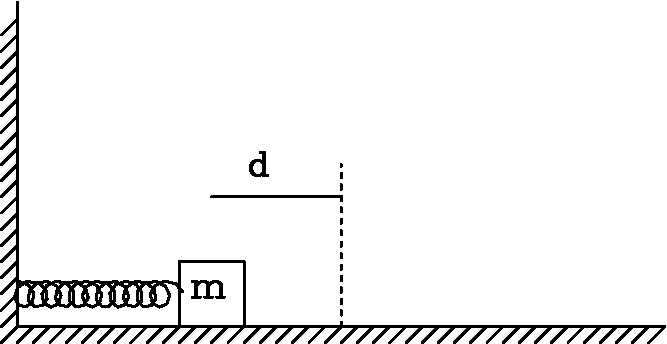
\includegraphics[width=0.25\textwidth]{4a-crop.pdf}\hspace{0.1\textwidth}
	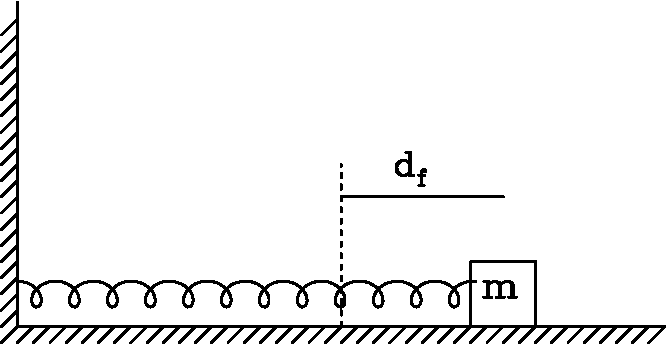
\includegraphics[width=0.25\textwidth]{4b-crop.pdf}
}


a) How fast will the mass be traveling when it crosses the equilibrium point? Give your answer in terms of $\mu_k$, $d$, $m$, and $g$. 

\vspace{1in}

b) Write down an expression for the work done by friction as the block slides from its starting point to the final position $d_f$ to the right of equilibrium. 

\vspace{1in}

c) Write down an equation in terms of $\mu_k$, $d$, $m$, and $g$ that will let you solve for the distance $d_f$. You do not need to solve it. 

\vspace{1in}

d) What algebraic technique would you have to use to solve this equation for $d_f$?




 \end{document}
